\section[For- and Background]{For- and Background}



\subsection{Certification Process}

\begin{frame}
  \frametitle{Strategy}
  When conceiving a Certification Strategy the different views are in our mind.
  
\end{frame}

\begin{frame}
 \frametitle{Selecting Questions}
 \begin{columns}
    \begin{column}{.5\textwidth}
       \centering
      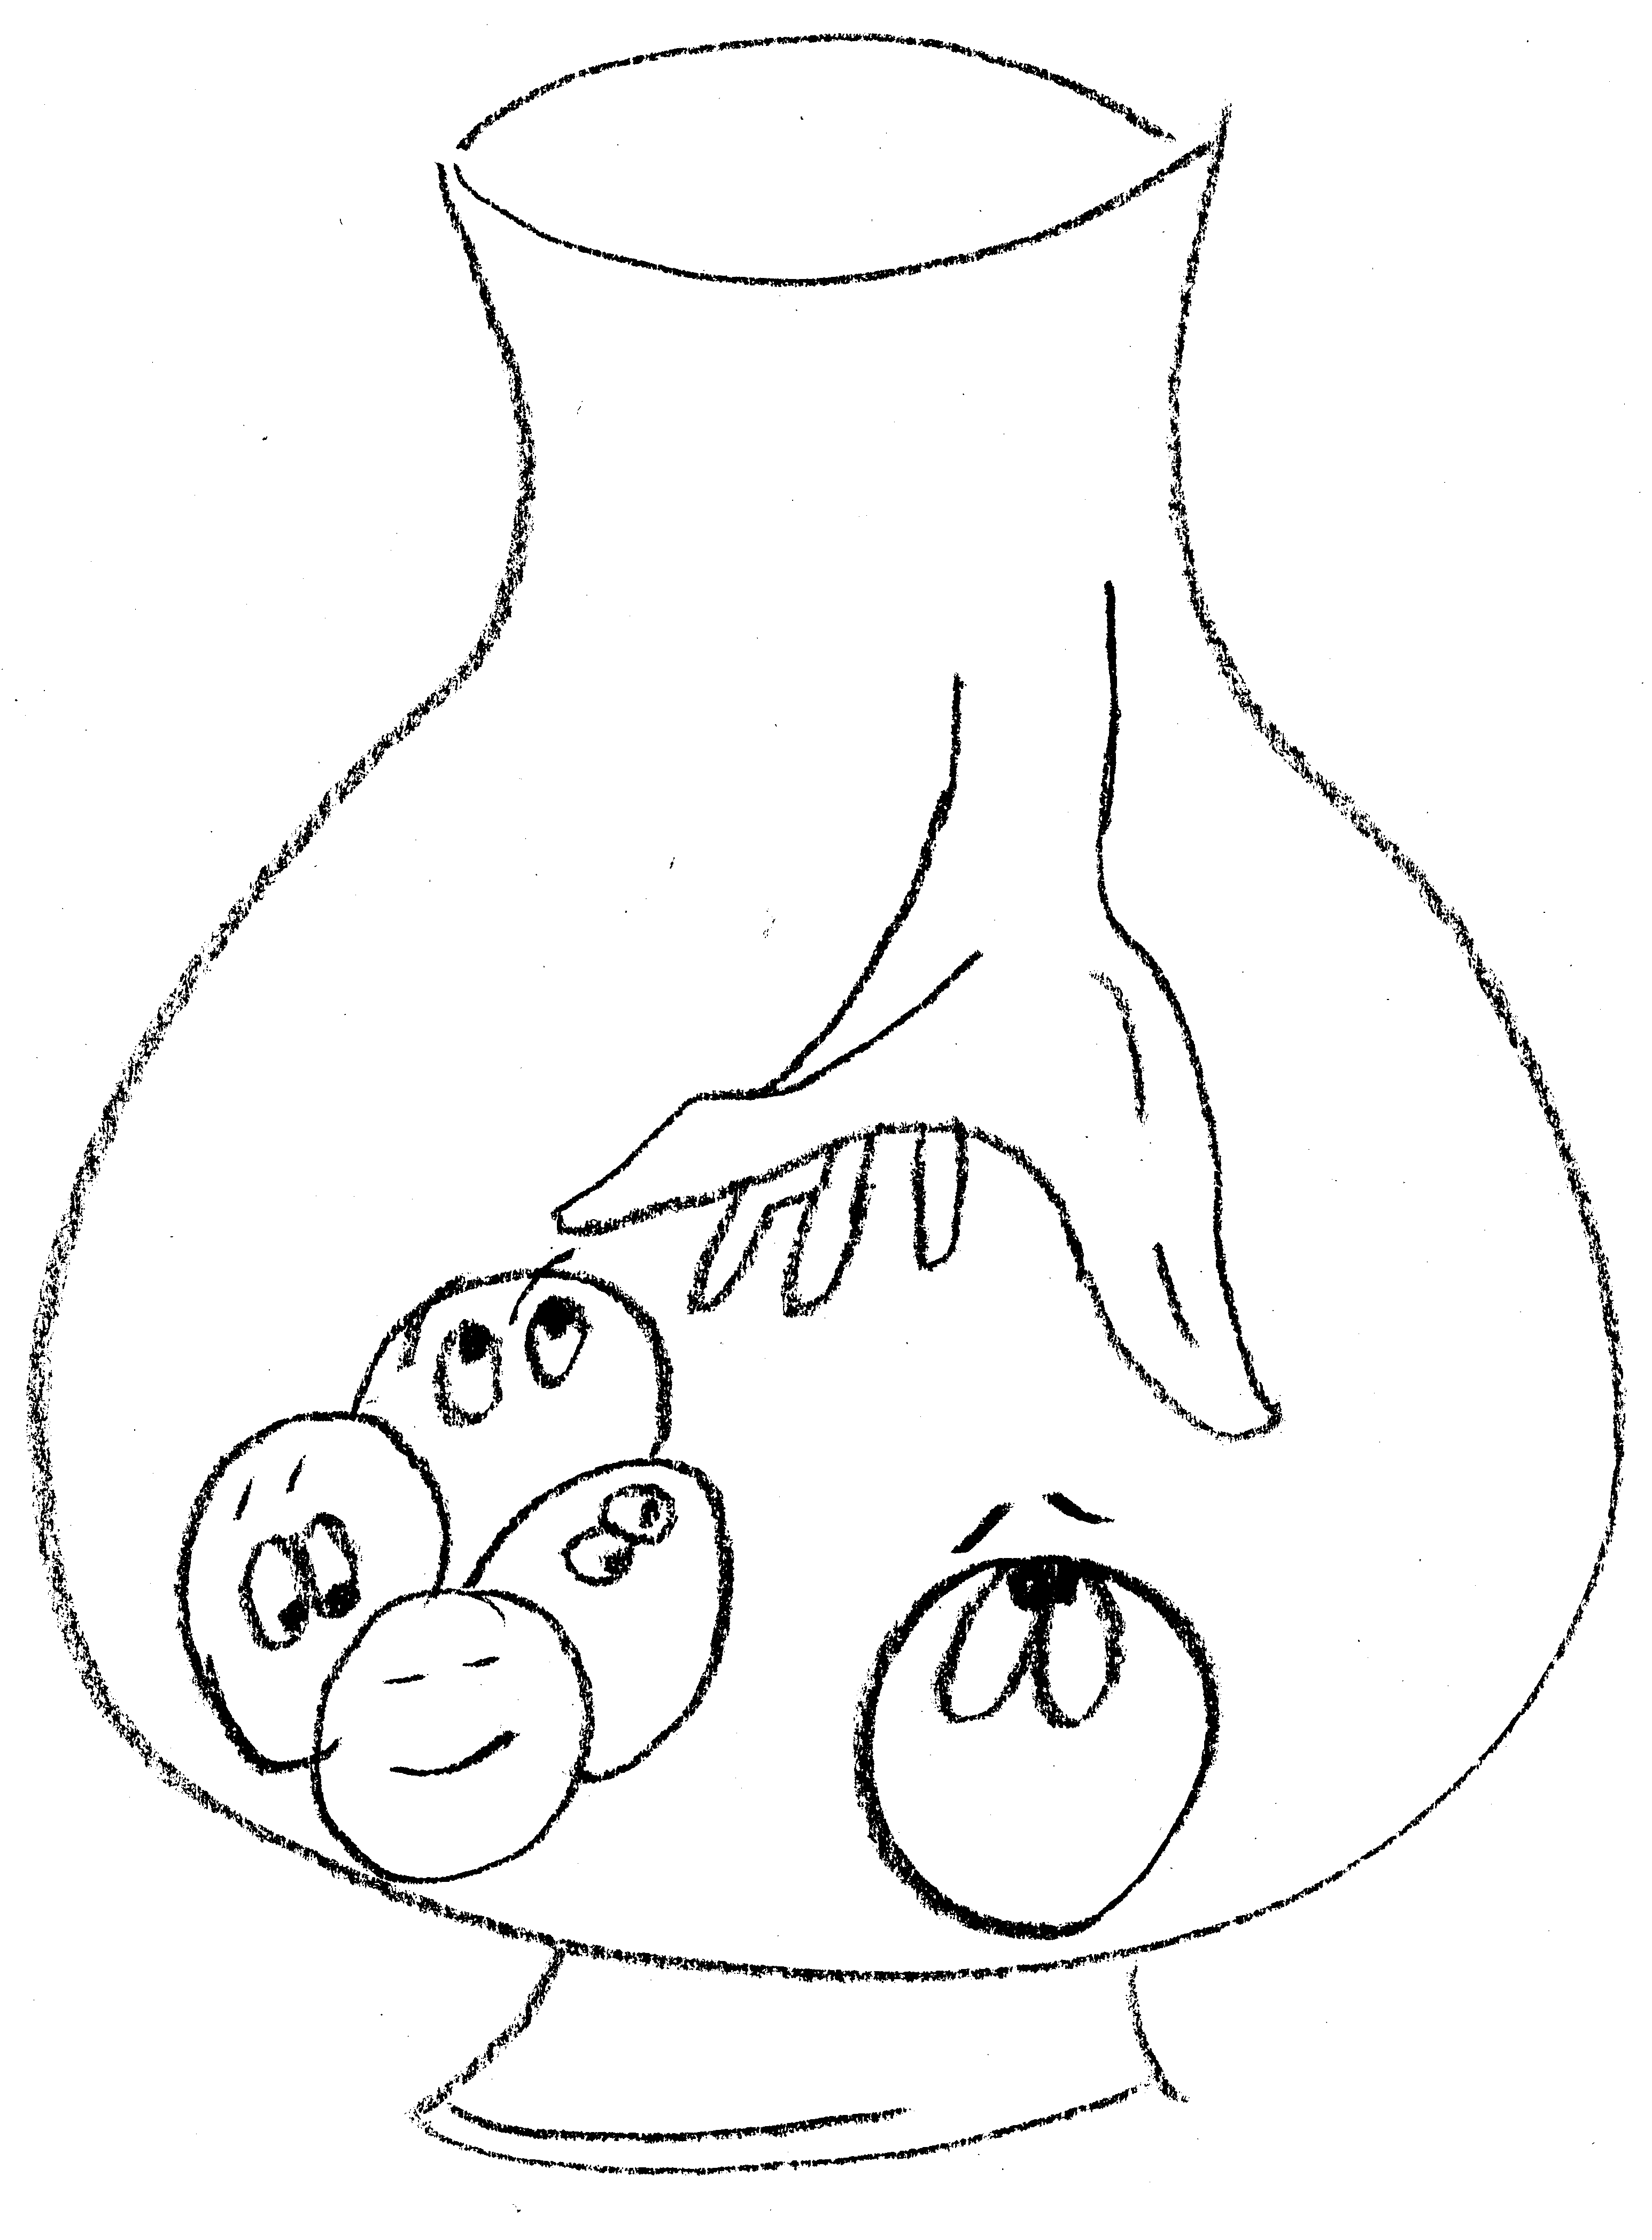
\includegraphics[width=0.6\textwidth]{images/urn}
    \end{column}
    \begin{column}{.5\textwidth}
      Questions are randomly choosen from a pool:
         the pool may itself be a bundle of sub-branches of the skill tree
              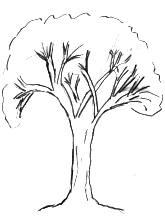
\includegraphics[width=0.1\textwidth]{images/tree_tiny}
        
      $\curvearrowright$ All examininations will be based on different sets of questions.
    \end{column}
  \end{columns}
\end{frame}

\begin{frame}
  \frametitle{On Cheating}
  \begin{columns}
   \begin{column}{.5\textwidth}
     \begin{enumerate}
      \item By confronting with random questions no perfect preperation can be accomplished.
      \item There is a time-limit per question.
      \item A registration prior to a test session is required.
     \end{enumerate}
    No online system without ID checks and other measures is safe against cheating! Yet, our measures will raise awareness.
   \end{column}
   \begin{column}{.5\textwidth}
       \centering
      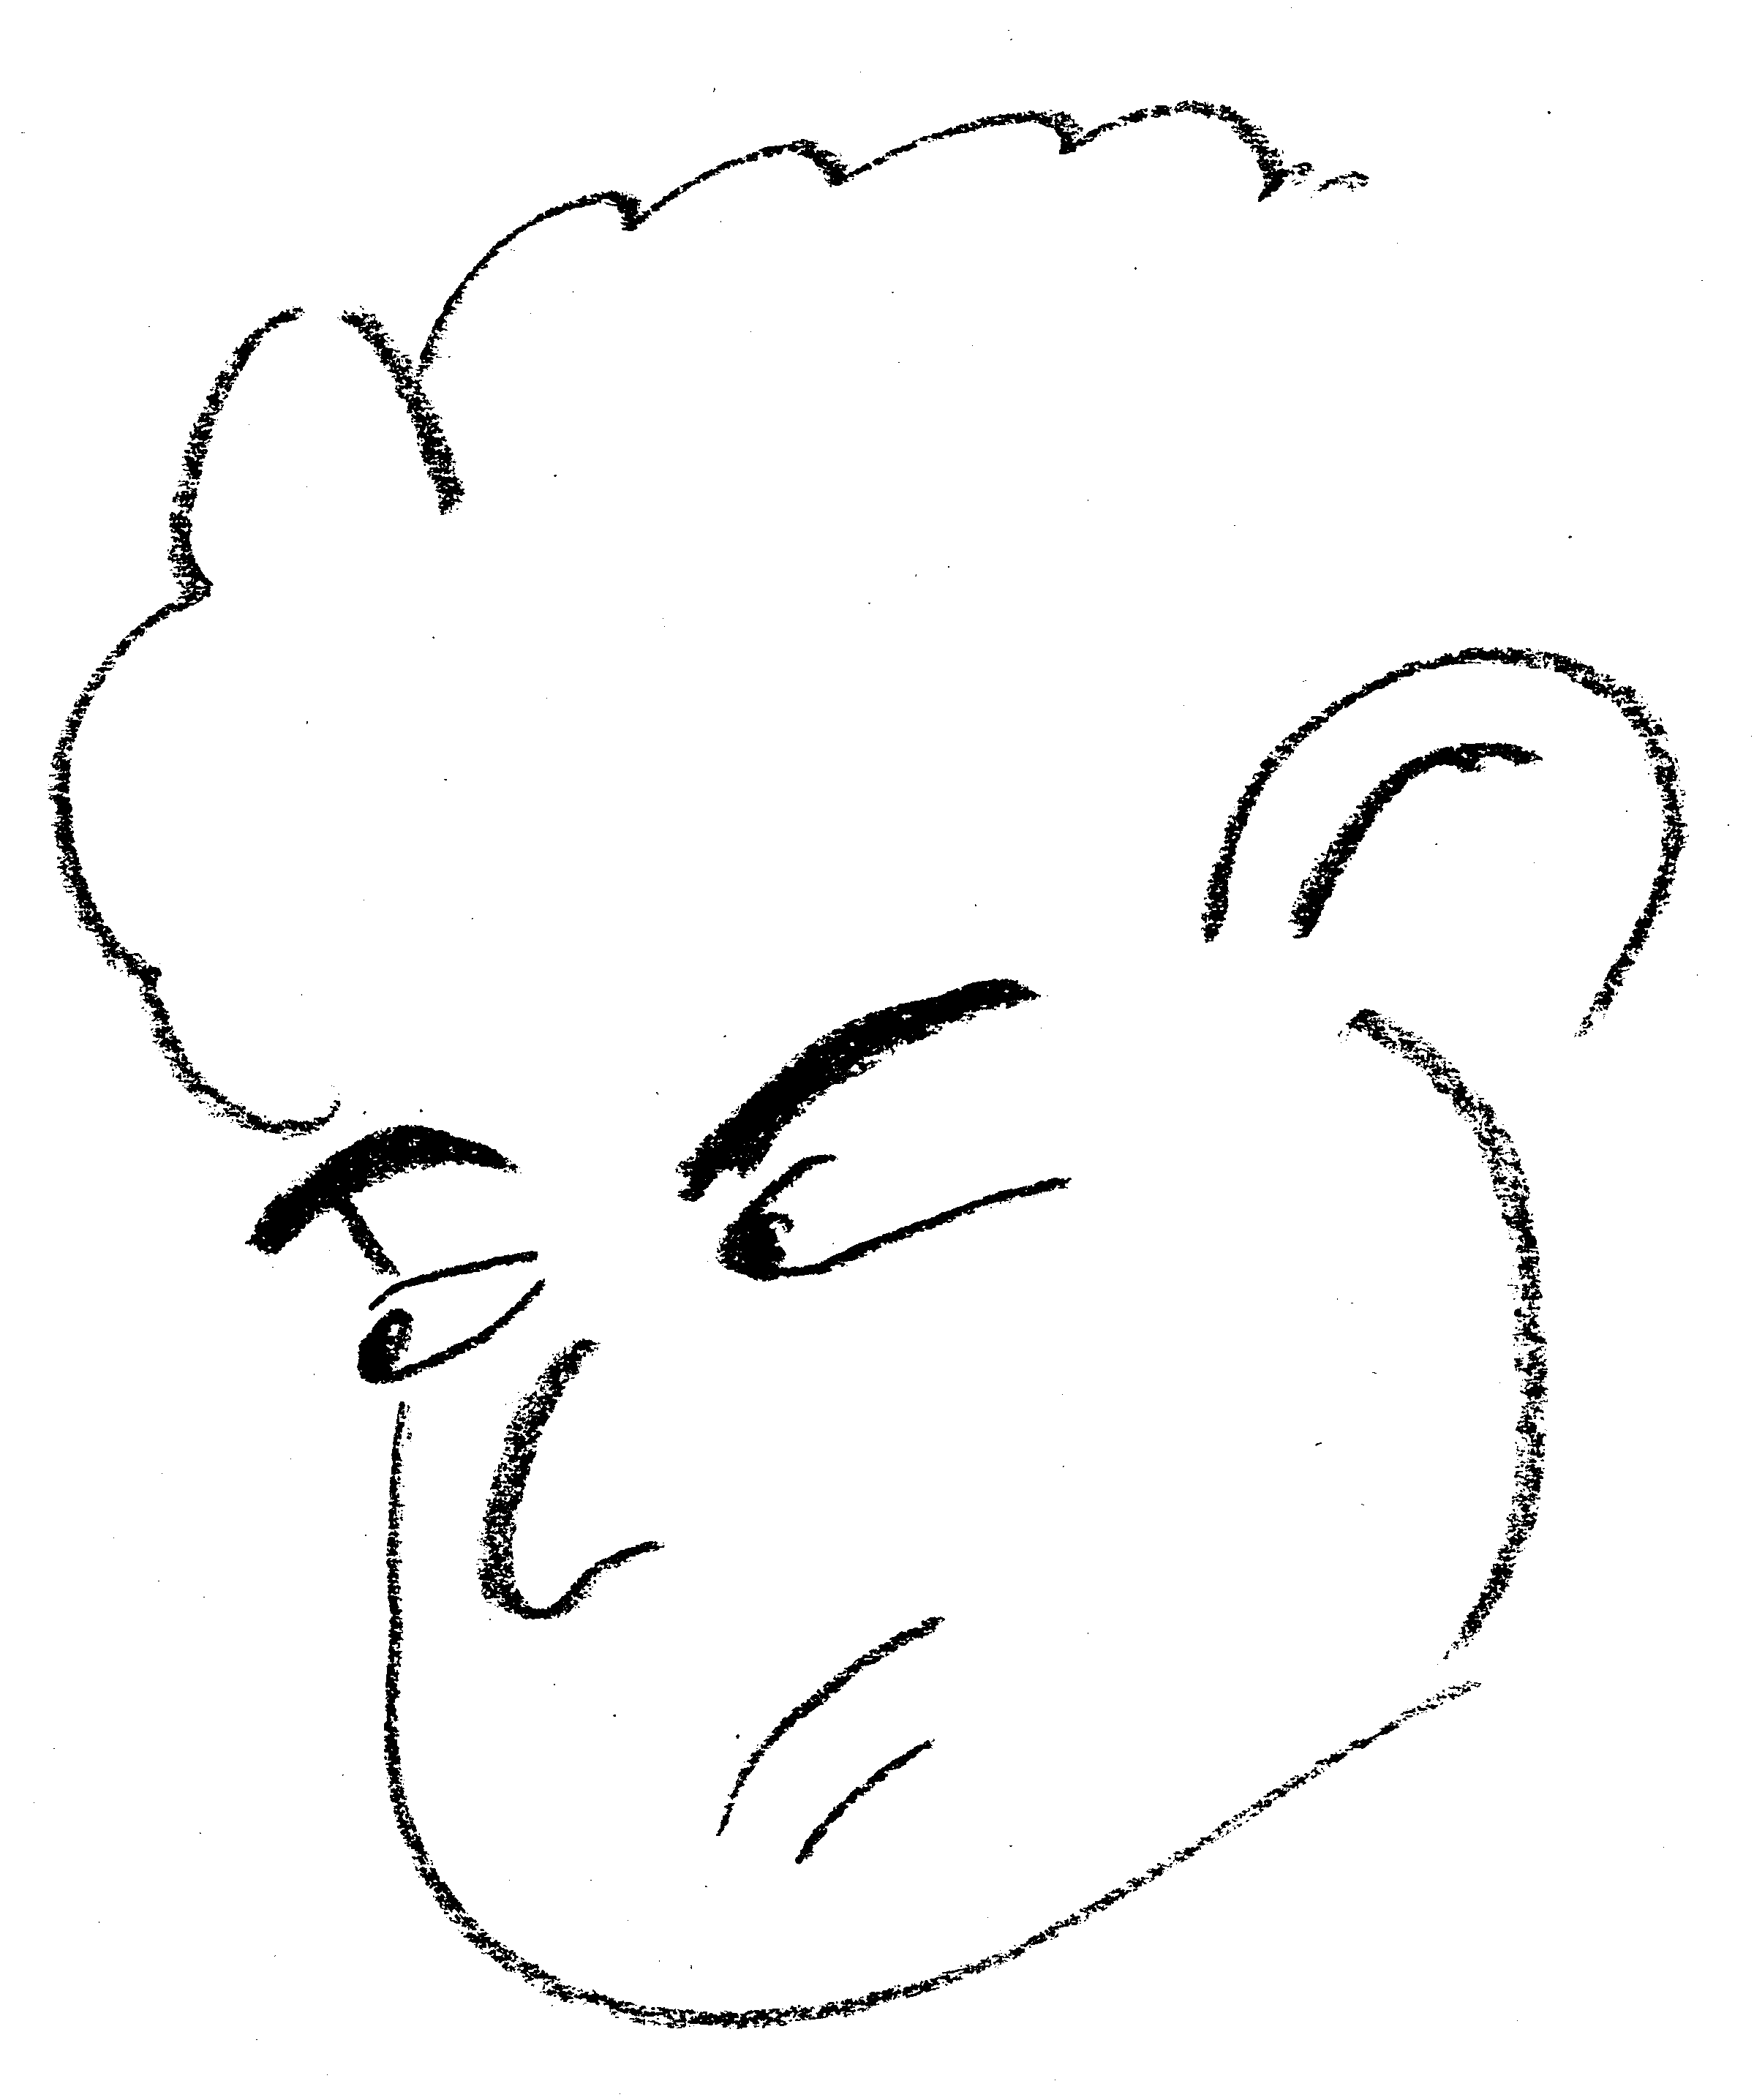
\includegraphics[width=0.6\textwidth]{images/cheating}
    \end{column}
  \end{columns}
\end{frame}

\begin{frame}
 \frametitle{Boosting Acceptance}
 \begin{columns}
   \begin{column}{.5\textwidth}
     Want to hire a scientist? \newline
     We intend to provide a (sub)set of question for prospective employers. This way they will have an idea of the background, if a solicitant waves a HPCCF-certificate.
   \end{column}
   \begin{column}{.5\textwidth}
       \centering
      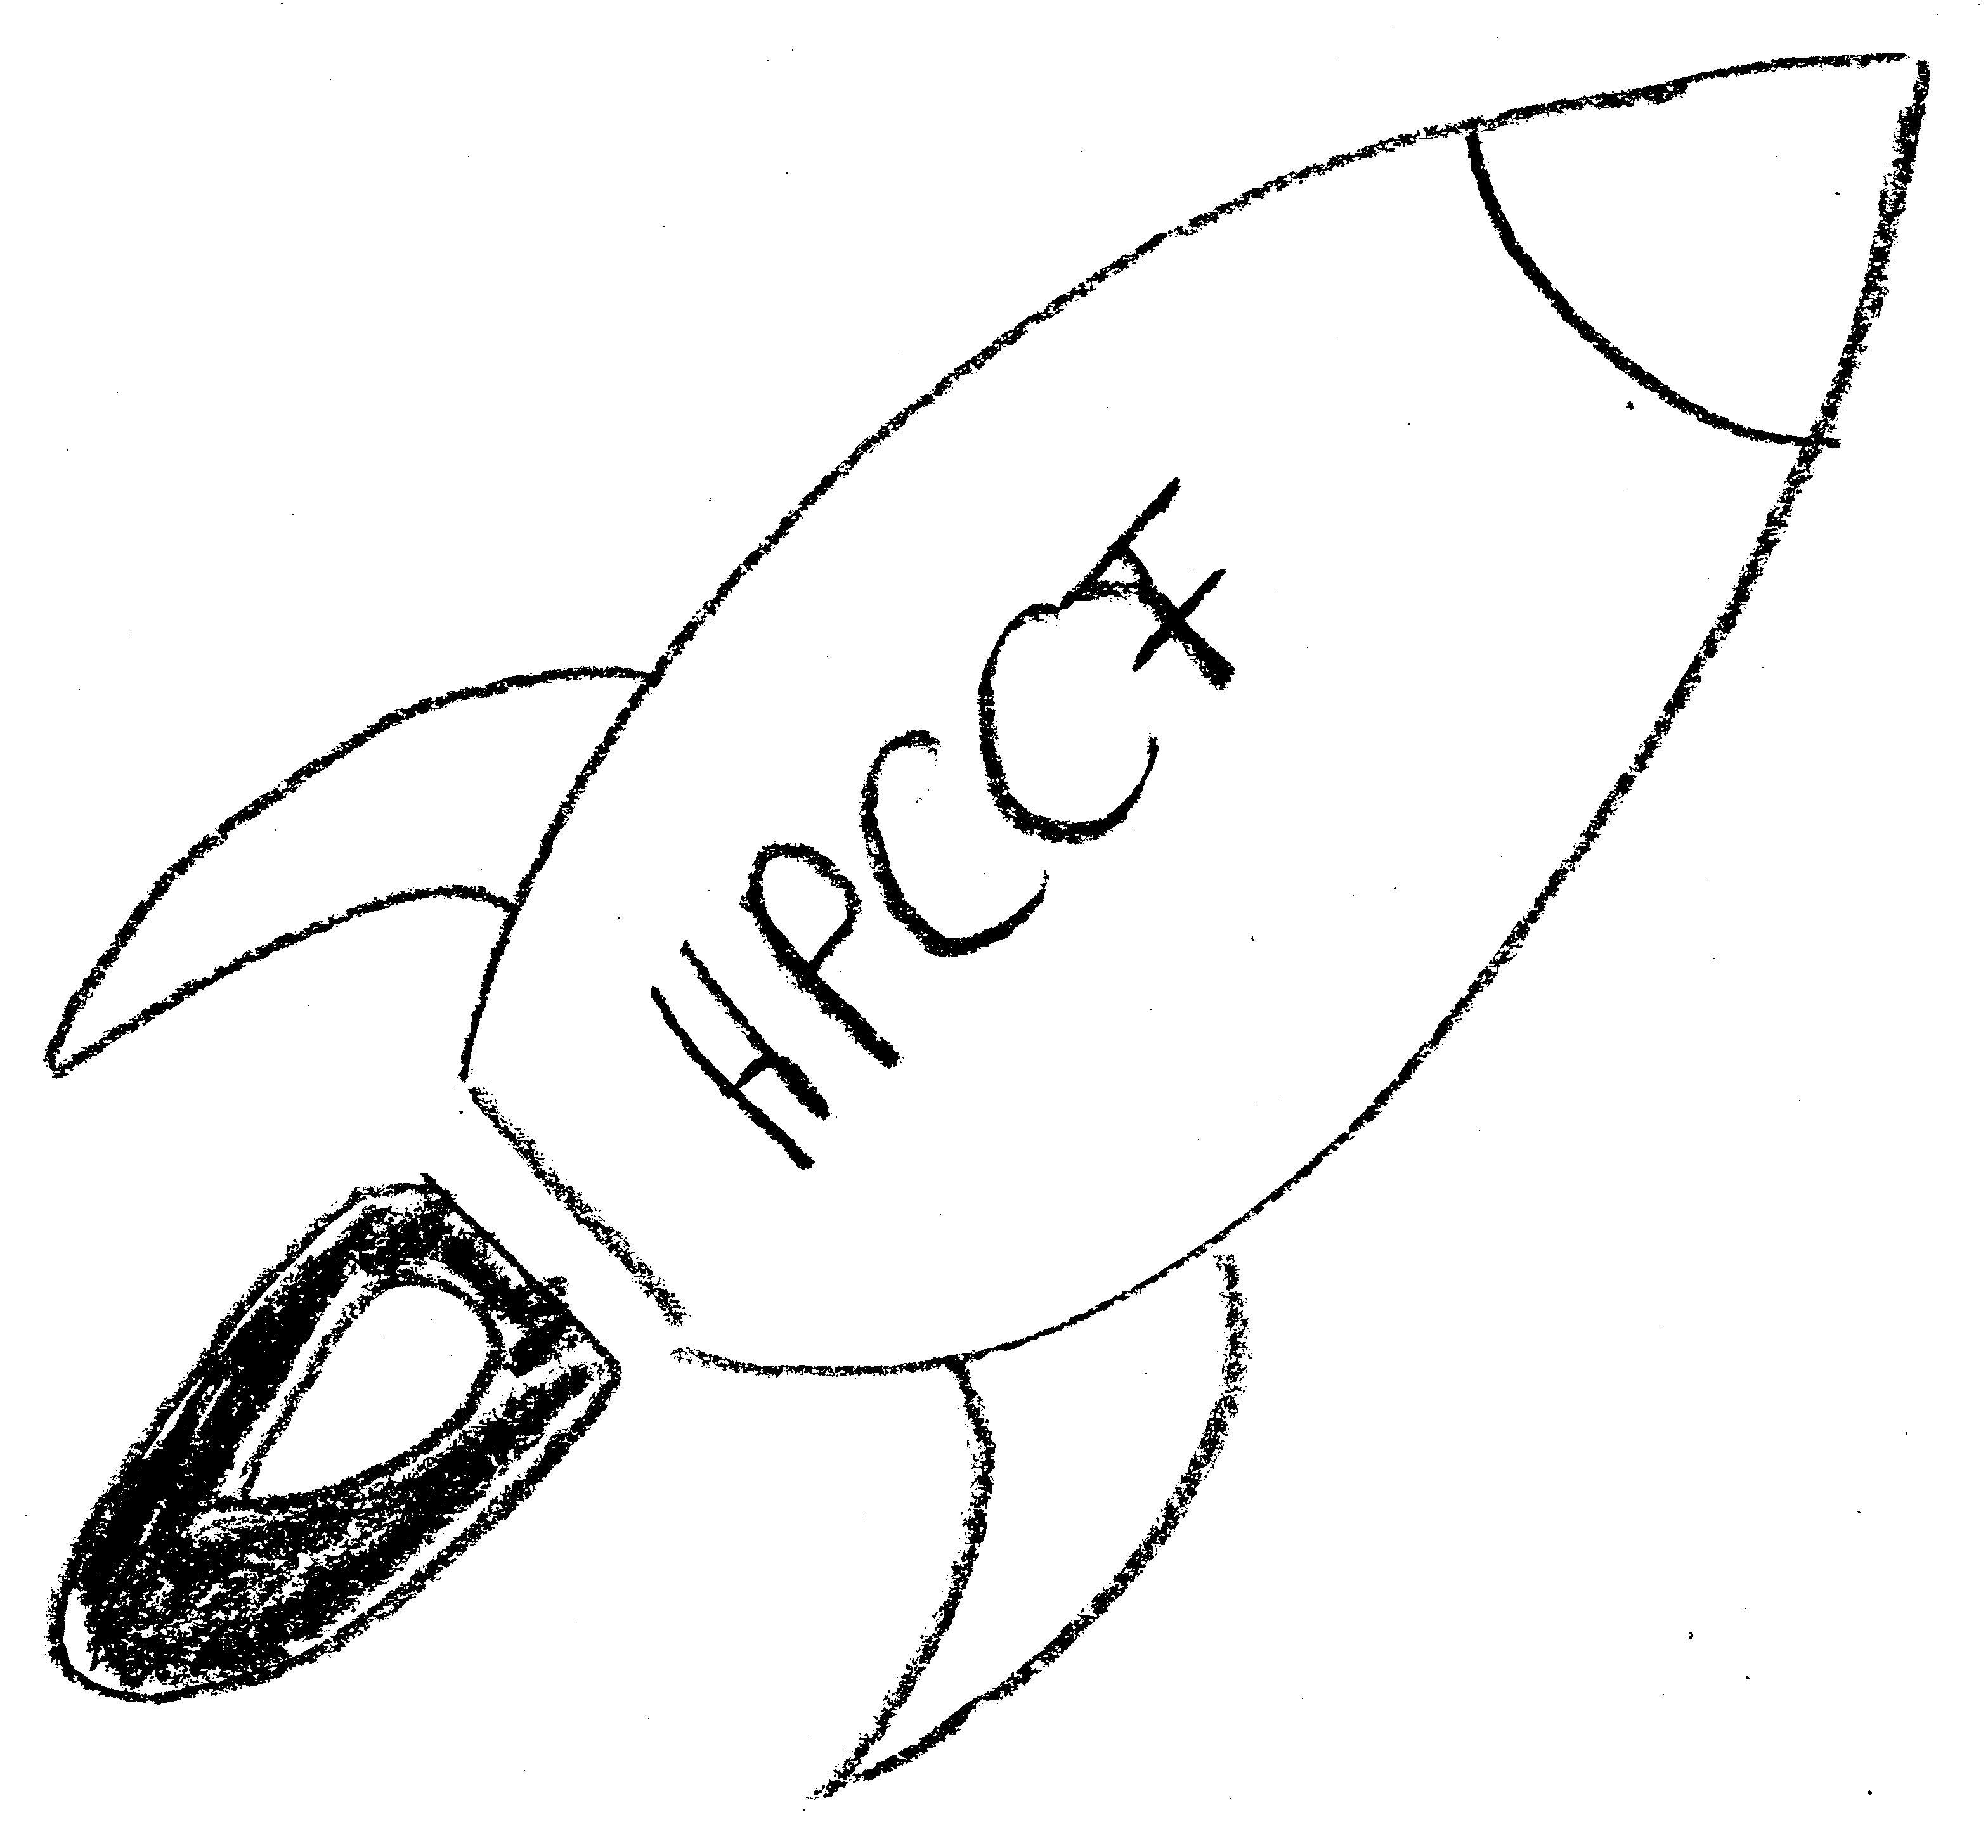
\includegraphics[width=0.6\textwidth]{images/hpccf_boost}
    \end{column}
  \end{columns}
\end{frame}




